\documentclass{standalone}
\usepackage{tikz}
\usetikzlibrary{patterns, positioning}
\usepackage[sfdefault]{ClearSans} %% option 'sfdefault' activates Clear Sans as the default text font
\usepackage[T1]{fontenc}

\begin{document}
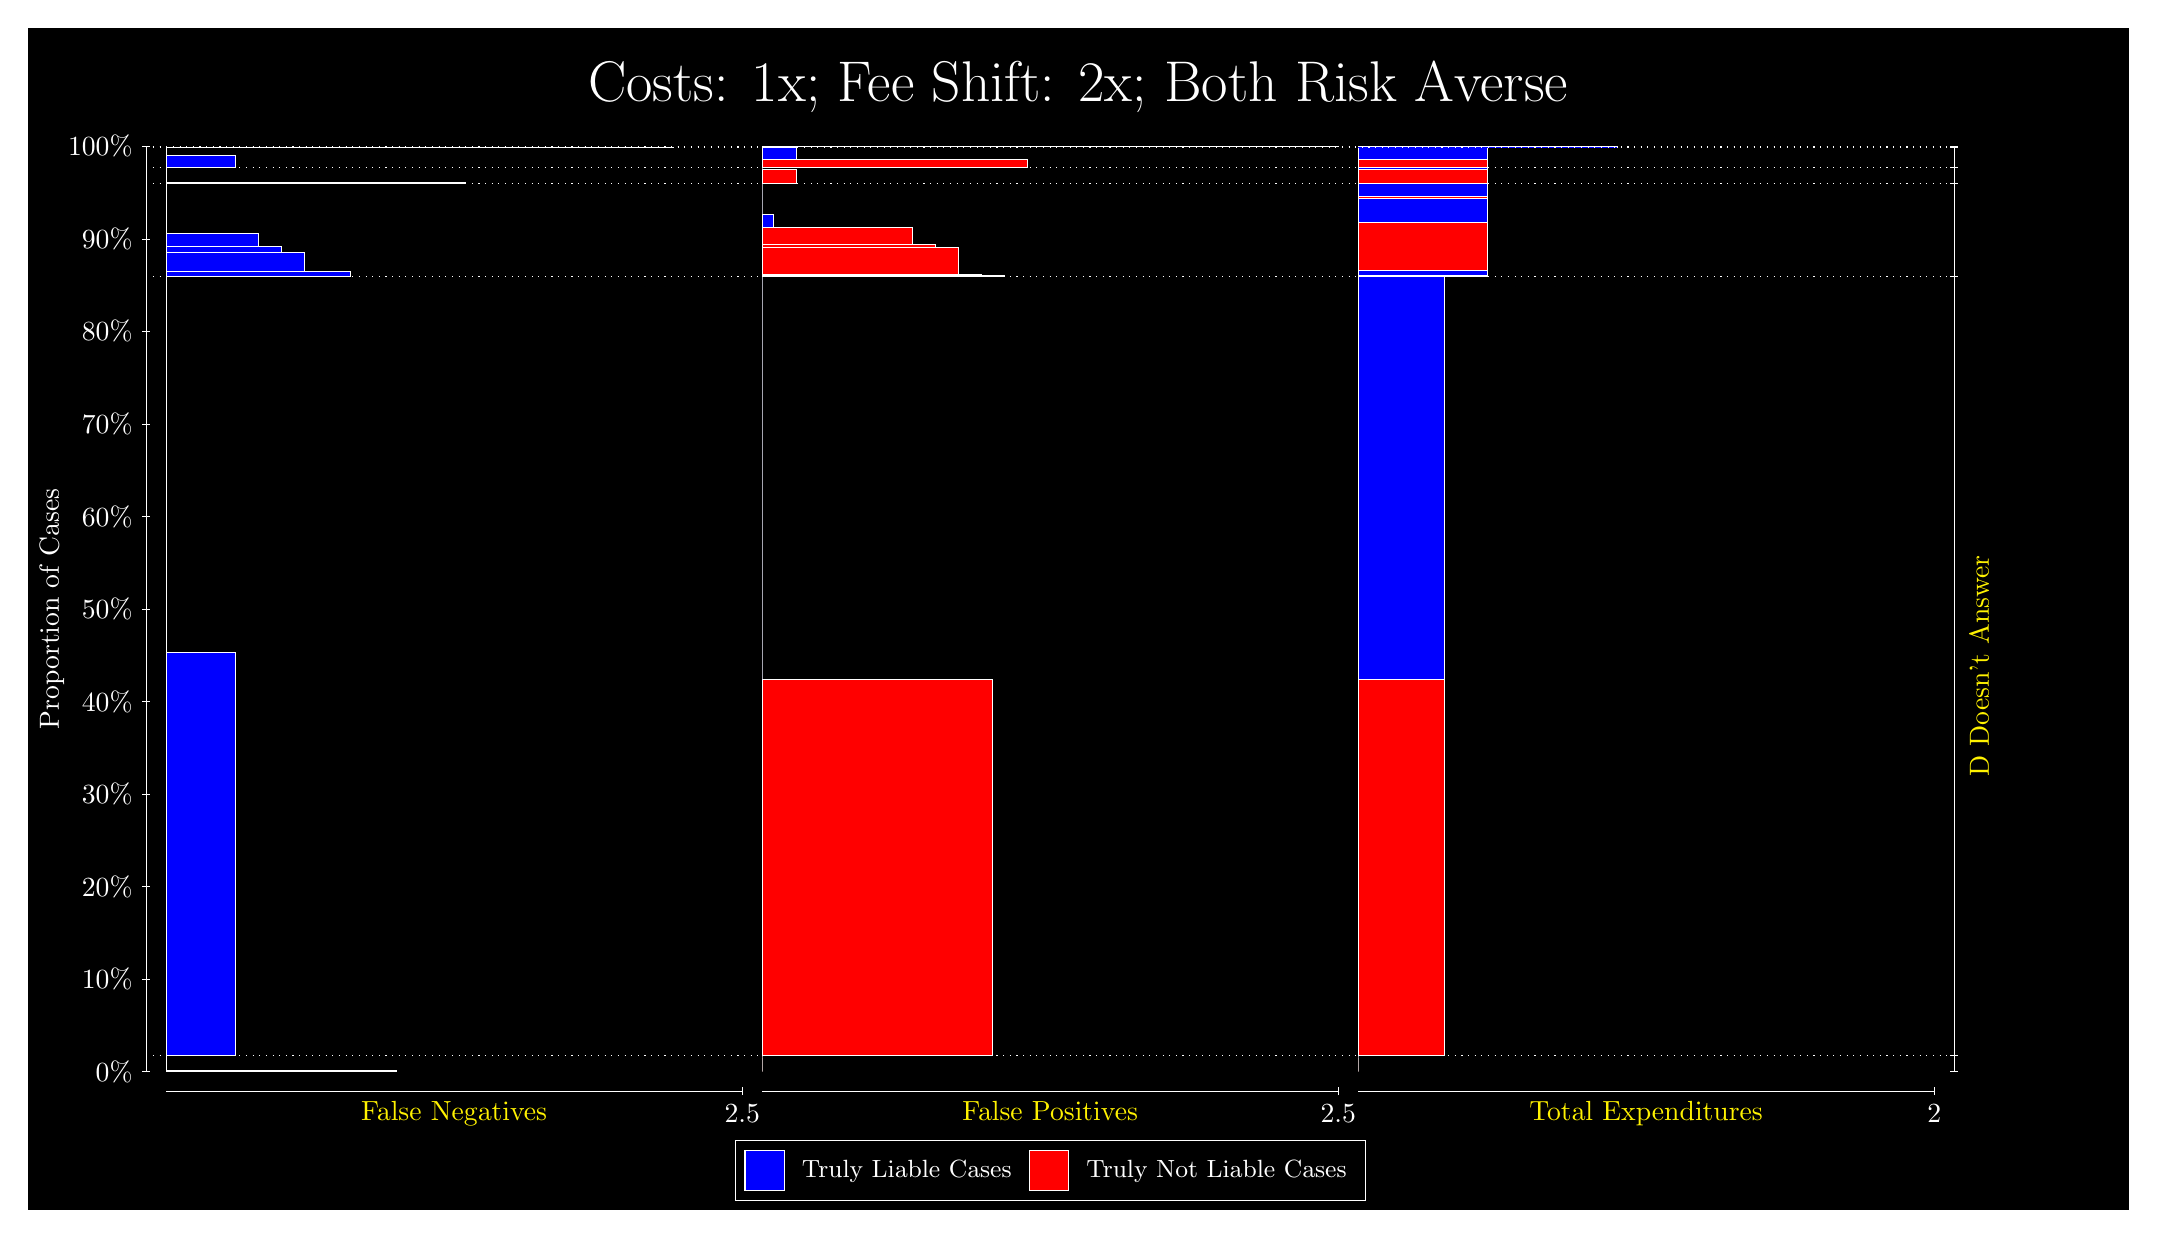
\begin{tikzpicture}
\draw[fill=black] (0,0) rectangle (26.667,15);
\draw[text=white] (0,13.5) rectangle (26.667,15) node[midway] {\huge Costs: 1x; Fee Shift: 2x; Both Risk Averse};
\draw[white, very thin] (1.5,1.75) -- (1.5,13.5);
\node[rotate=90, text=white, anchor=center] at (0.3, 7.625) {Proportion of Cases};
\draw[white, very thin] (1.45,1.75) -- (1.55,1.75);
\node[text=white, anchor=east] at (1.45, 1.75) {0\%};
\draw[white, very thin] (1.45,2.925) -- (1.55,2.925);
\node[text=white, anchor=east] at (1.45, 2.925) {10\%};
\draw[white, very thin] (1.45,4.1) -- (1.55,4.1);
\node[text=white, anchor=east] at (1.45, 4.1) {20\%};
\draw[white, very thin] (1.45,5.275) -- (1.55,5.275);
\node[text=white, anchor=east] at (1.45, 5.275) {30\%};
\draw[white, very thin] (1.45,6.45) -- (1.55,6.45);
\node[text=white, anchor=east] at (1.45, 6.45) {40\%};
\draw[white, very thin] (1.45,7.625) -- (1.55,7.625);
\node[text=white, anchor=east] at (1.45, 7.625) {50\%};
\draw[white, very thin] (1.45,8.8) -- (1.55,8.8);
\node[text=white, anchor=east] at (1.45, 8.8) {60\%};
\draw[white, very thin] (1.45,9.975) -- (1.55,9.975);
\node[text=white, anchor=east] at (1.45, 9.975) {70\%};
\draw[white, very thin] (1.45,11.15) -- (1.55,11.15);
\node[text=white, anchor=east] at (1.45, 11.15) {80\%};
\draw[white, very thin] (1.45,12.325) -- (1.55,12.325);
\node[text=white, anchor=east] at (1.45, 12.325) {90\%};
\draw[white, very thin] (1.45,13.5) -- (1.55,13.5);
\node[text=white, anchor=east] at (1.45, 13.5) {100\%};

\draw[white, very thin] (24.457,1.75) -- (24.457,13.5);
\draw[white, very thin] (24.407,1.75) -- (24.507,1.75);
\node[anchor=west] at (24.407, 1.75) {};
\draw[white, very thin] (24.407,1.9526) -- (24.507,1.9526);
\node[anchor=west] at (24.407, 1.9526) {};
\draw[white, very thin] (24.407,11.845) -- (24.507,11.845);
\node[anchor=west] at (24.407, 11.845) {};
\draw[white, very thin] (24.407,13.025) -- (24.507,13.025);
\node[anchor=west] at (24.407, 13.025) {};
\draw[white, very thin] (24.407,13.229) -- (24.507,13.229);
\node[anchor=west] at (24.407, 13.229) {};
\draw[white, very thin] (24.407,13.492) -- (24.507,13.492);
\node[anchor=west] at (24.407, 13.492) {};
\draw[white, very thin] (24.407,13.497) -- (24.507,13.497);
\node[anchor=west] at (24.407, 13.497) {};
\draw[white, very thin] (24.407,13.5) -- (24.507,13.5);
\node[anchor=west] at (24.407, 13.5) {};

\draw[white, very thin, fill=blue] (1.75,1.75) rectangle (4.6775,1.7713);
\draw[white, very thin, fill=red] (1.75,1.7713) rectangle (1.75,1.9526);
\draw[white, very thin, fill=blue] (1.75,1.9526) rectangle (2.6283,7.0703);
\draw[white, very thin, fill=red] (1.75,7.0703) rectangle (1.75,11.845);
\draw[white, very thin, fill=blue] (1.75,11.845) rectangle (4.092,11.914);
\draw[white, very thin, fill=blue] (1.75,11.914) rectangle (3.7993,11.917);
\draw[white, very thin, fill=blue] (1.75,11.917) rectangle (3.5065,12.156);
\draw[white, very thin, fill=blue] (1.75,12.156) rectangle (3.2138,12.23);
\draw[white, very thin, fill=blue] (1.75,12.23) rectangle (2.921,12.394);
\draw[white, very thin, fill=red] (1.75,12.394) rectangle (1.75,13.025);
\draw[white, very thin, fill=blue] (1.75,13.025) rectangle (5.5558,13.048);
\draw[white, very thin, fill=red] (1.75,13.048) rectangle (1.75,13.229);
\draw[white, very thin, fill=blue] (1.75,13.229) rectangle (2.6283,13.391);
\draw[white, very thin, fill=red] (1.75,13.391) rectangle (1.75,13.492);
\draw[white, very thin, fill=blue] (1.75,13.492) rectangle (8.1906,13.493);
\draw[white, very thin, fill=red] (1.75,13.493) rectangle (1.75,13.497);
\draw[white, very thin, fill=red] (1.75,13.497) rectangle (1.75,13.499);
\draw[white, very thin, fill=blue] (1.75,13.499) rectangle (1.75,13.5);
\draw[white, very thin, fill=red] (9.3189,1.75) rectangle (9.3189,1.9313);
\draw[white, very thin, fill=blue] (9.3189,1.9313) rectangle (9.3189,1.9526);
\draw[white, very thin, fill=red] (9.3189,1.9526) rectangle (12.246,6.7278);
\draw[white, very thin, fill=blue] (9.3189,6.7278) rectangle (9.3189,11.845);
\draw[white, very thin, fill=red] (9.3189,11.845) rectangle (12.393,11.866);
\draw[white, very thin, fill=red] (9.3189,11.866) rectangle (12.1,11.877);
\draw[white, very thin, fill=red] (9.3189,11.877) rectangle (11.807,12.223);
\draw[white, very thin, fill=red] (9.3189,12.223) rectangle (11.515,12.254);
\draw[white, very thin, fill=red] (9.3189,12.254) rectangle (11.222,12.476);
\draw[white, very thin, fill=blue] (9.3189,12.476) rectangle (9.4652,12.64);
\draw[white, very thin, fill=blue] (9.3189,12.64) rectangle (9.3189,13.025);
\draw[white, very thin, fill=red] (9.3189,13.025) rectangle (9.758,13.206);
\draw[white, very thin, fill=blue] (9.3189,13.206) rectangle (9.3189,13.229);
\draw[white, very thin, fill=red] (9.3189,13.229) rectangle (12.686,13.33);
\draw[white, very thin, fill=blue] (9.3189,13.33) rectangle (9.758,13.492);
\draw[white, very thin, fill=red] (9.3189,13.492) rectangle (9.3189,13.496);
\draw[white, very thin, fill=blue] (9.3189,13.496) rectangle (9.3189,13.497);
\draw[white, very thin, fill=red] (9.3189,13.497) rectangle (16.638,13.499);
\draw[white, very thin, fill=blue] (9.3189,13.499) rectangle (13.71,13.5);
\draw[white, very thin, fill=red] (16.888,1.75) rectangle (16.888,1.9313);
\draw[white, very thin, fill=blue] (16.888,1.9313) rectangle (16.888,1.9526);
\draw[white, very thin, fill=red] (16.888,1.9526) rectangle (17.986,6.7278);
\draw[white, very thin, fill=blue] (16.888,6.7278) rectangle (17.986,11.845);
\draw[white, very thin, fill=red] (16.888,11.845) rectangle (18.534,11.857);
\draw[white, very thin, fill=blue] (16.888,11.857) rectangle (18.534,11.931);
\draw[white, very thin, fill=red] (16.888,11.931) rectangle (18.534,12.53);
\draw[white, very thin, fill=blue] (16.888,12.53) rectangle (18.534,12.84);
\draw[white, very thin, fill=red] (16.888,12.84) rectangle (18.534,12.86);
\draw[white, very thin, fill=blue] (16.888,12.86) rectangle (18.534,13.025);
\draw[white, very thin, fill=red] (16.888,13.025) rectangle (18.534,13.206);
\draw[white, very thin, fill=blue] (16.888,13.206) rectangle (18.534,13.229);
\draw[white, very thin, fill=red] (16.888,13.229) rectangle (18.534,13.33);
\draw[white, very thin, fill=blue] (16.888,13.33) rectangle (18.534,13.492);
\draw[white, very thin, fill=red] (16.888,13.492) rectangle (20.181,13.496);
\draw[white, very thin, fill=blue] (16.888,13.496) rectangle (20.181,13.497);
\draw[white, very thin, fill=red] (16.888,13.497) rectangle (20.181,13.499);
\draw[white, very thin, fill=blue] (16.888,13.499) rectangle (20.181,13.5);
\draw[white, dotted] (1.5,1.9526) -- (24.457,1.9526);
\draw[white, dotted] (1.5,11.845) -- (24.457,11.845);
\draw[white, dotted] (1.5,13.025) -- (24.457,13.025);
\draw[white, dotted] (1.5,13.229) -- (24.457,13.229);
\draw[white, dotted] (1.5,13.492) -- (24.457,13.492);
\draw[white, dotted] (1.5,13.497) -- (24.457,13.497);
\draw[white, very thin] (1.75,1.5) -- (9.0689,1.5);
\node[text=yellow, anchor=north] at (5.4094, 1.5) {False Negatives};
\draw[white, very thin] (9.0689,1.45) -- (9.0689,1.55);
\node[text=white, anchor=north] at (9.0689, 1.45) {2.5};

\draw[white, very thin] (9.3189,1.5) -- (16.638,1.5);
\node[text=yellow, anchor=north] at (12.978, 1.5) {False Positives};
\draw[white, very thin] (16.638,1.45) -- (16.638,1.55);
\node[text=white, anchor=north] at (16.638, 1.45) {2.5};

\draw[white, very thin] (16.888,1.5) -- (24.207,1.5);
\node[text=yellow, anchor=north] at (20.547, 1.5) {Total Expenditures};
\draw[white, very thin] (24.207,1.45) -- (24.207,1.55);
\node[text=white, anchor=north] at (24.207, 1.45) {2};


\node[text=yellow, centered, rotate=90] at (24.777, 6.899) {D Doesn't Answer};






\draw (12.978300999999998,1.5) node[draw=none] (baseCoordinate) {};
\begin{scope}[align=center]
        \matrix[scale=0.5, draw=white, below=0.5cm of baseCoordinate, nodes={draw}, column sep=0.1cm]{
            \node[rectangle, draw, minimum width=0.5cm, minimum height=0.5cm, fill=blue] {}; &
            \node[draw=none, font=\small, text=white] (B) {Truly Liable Cases}; &
            \node[rectangle, draw, minimum width=0.5cm, minimum height=0.5cm, fill=red] {}; &
            \node[draw=none, font=\small, text=white] (B) {Truly Not Liable Cases}; \\
            };
\end{scope}

\end{tikzpicture}
\end{document}